% !TeX TXS-program:bibliography = txs:///biber
\documentclass[14pt, russian]{scrartcl}
\let\counterwithout\relax
\let\counterwithin\relax
%\usepackage{lmodern}
\usepackage{float}
\usepackage{xcolor}
\usepackage{extsizes}
\usepackage{subfig}
\usepackage[export]{adjustbox}
\usepackage{tocvsec2} % возможность менять учитываемую глубину разделов в оглавлении
\usepackage[subfigure]{tocloft}
\usepackage[newfloat]{minted}
\captionsetup[listing]{position=top}

\AtBeginEnvironment{figure}{\vspace{0.5cm}}
\AtBeginEnvironment{table}{\vspace{0.5cm}}
\AtBeginEnvironment{listing}{\vspace{0.5cm}}
\AtBeginEnvironment{algorithm}{\vspace{0.5cm}}
\AtBeginEnvironment{minted}{\vspace{-0.5cm}}

\usepackage{fancyvrb}
\usepackage{ulem,bm,mathrsfs,ifsym} %зачеркивания, особо жирный стиль и RSFS начертание
\usepackage{sectsty} % переопределение стилей подразделов
\usepackage{caption} % для многостраничных листингов будет создано новое окружение 
%%%%%%%%%%%%%%%%%%%%%%%

%%% Поля и разметка страницы %%%
\usepackage{pdflscape}                              % Для включения альбомных страниц
\usepackage{geometry}                               % Для последующего задания полей
\geometry{a4paper,tmargin=2cm,bmargin=2cm,lmargin=3cm,rmargin=1cm} % тоже самое, но лучше

%%% Математические пакеты %%%
\usepackage{amsthm,amsfonts,amsmath,amssymb,amscd}  % Математические дополнения от AMS
\usepackage{mathtools}                              % Добавляет окружение multlined
\usepackage[perpage]{footmisc}
%\usepackage{times}

%%%% Установки для размера шрифта 14 pt %%%%
%% Формирование переменных и констант для сравнения (один раз для всех подключаемых файлов)%%
%% должно располагаться до вызова пакета fontspec или polyglossia, потому что они сбивают его работу
%\newlength{\curtextsize}
%\newlength{\bigtextsize}
%\setlength{\bigtextsize}{13pt}
\KOMAoptions{fontsize=14pt}

\makeatletter
\def\showfontsize{\f@size{} point}
\makeatother

%\makeatletter
%\show\f@size                                       % неплохо для отслеживания, но вызывает стопорение процесса, если документ компилируется без команды  -interaction=nonstopmode 
%\setlength{\curtextsize}{\f@size pt}
%\makeatother

%шрифт times
\usepackage{tempora} %только для тех, у кого MikTeX последней версии и не ловит pscyr
%\usepackage{pscyr} %для всех нормальных людей
%\setmainfont[Ligatures={TeX,Historic}]{Times New Roman}

   %%% Решение проблемы копирования текста в буфер кракозябрами
%    \input glyphtounicode.tex
%    \input glyphtounicode-cmr.tex %from pdfx package
%    \pdfgentounicode=1
    \usepackage{cmap}                               % Улучшенный поиск русских слов в полученном pdf-файле
    \usepackage[T1]{fontenc}                       % Поддержка русских букв
    \usepackage[utf8]{inputenc}                     % Кодировка utf8
    \usepackage[english, main=russian]{babel}            % Языки: русский, английский
%   \IfFileExists{pscyr.sty}{\usepackage{pscyr}}{}  % Красивые русские шрифты
%\renewcommand{\rmdefault}{ftm}
%%% Оформление абзацев %%%
\usepackage{indentfirst}                            % Красная строка
%\usepackage{eskdpz}

%%% Таблицы %%%
\usepackage{longtable}                              % Длинные таблицы
\usepackage{multirow,makecell,array}                % Улучшенное форматирование таблиц
\usepackage{booktabs}                               % Возможность оформления таблиц в классическом книжном стиле (при правильном использовании не противоречит ГОСТ)

%%% Общее форматирование
\usepackage{soulutf8}                               % Поддержка переносоустойчивых подчёркиваний и зачёркиваний
\usepackage{icomma}                                 % Запятая в десятичных дробях



%%% Изображения %%%
\usepackage{graphicx}                               % Подключаем пакет работы с графикой
\usepackage{wrapfig}

%%% Списки %%%
\usepackage{enumitem}

%%% Подписи %%%
\usepackage{caption}                                % Для управления подписями (рисунков и таблиц) % Может управлять номерами рисунков и таблиц с caption %Иногда может управлять заголовками в списках рисунков и таблиц
%% Использование:
%\begin{table}[h!]\ContinuedFloat - чтобы не переключать счетчик
%\captionsetup{labelformat=continued}% должен стоять до самого caption
%\caption{}
% либо ручками \caption*{Продолжение таблицы~\ref{...}.} :)

\AtBeginEnvironment{minted}{%
  \renewcommand{\fcolorbox}[4][]{#4}}
  
%%% Интервалы %%%
\addto\captionsrussian{%
  \renewcommand{\listingname}{Листинг}%
}
%%% Счётчики %%%
\usepackage[figure,table,section]{totalcount}               % Счётчик рисунков и таблиц
\DeclareTotalCounter{lstlisting}
\usepackage{totcount}                               % Пакет создания счётчиков на основе последнего номера подсчитываемого элемента (может требовать дважды компилировать документ)
\usepackage{totpages}                               % Счётчик страниц, совместимый с hyperref (ссылается на номер последней страницы). Желательно ставить последним пакетом в преамбуле

%%% Продвинутое управление групповыми ссылками (пока только формулами) %%%
%% Кодировки и шрифты %%%

%   \newfontfamily{\cyrillicfont}{Times New Roman}
%   \newfontfamily{\cyrillicfonttt}{CMU Typewriter Text}
	%\setmainfont{Times New Roman}
	%\newfontfamily\cyrillicfont{Times New Roman}
	%\setsansfont{Times New Roman}                    %% задаёт шрифт без засечек
%	\setmonofont{Liberation Mono}               %% задаёт моноширинный шрифт
%    \IfFileExists{pscyr.sty}{\renewcommand{\rmdefault}{ftm}}{}
%%% Интервалы %%%
%linespread-реализация ближе к реализации полуторного интервала в ворде.
%setspace реализация заточена под шрифты 10, 11, 12pt, под остальные кегли хуже, но всё же ближе к типографской классике. 
\linespread{1.3}                    % Полуторный интервал (ГОСТ Р 7.0.11-2011, 5.3.6)
%\renewcommand{\@biblabel}[1]{#1}

%%% Гиперссылки %%%
\usepackage{hyperref}

%%% Выравнивание и переносы %%%
\sloppy                             % Избавляемся от переполнений
\clubpenalty=10000                  % Запрещаем разрыв страницы после первой строки абзаца
\widowpenalty=10000                 % Запрещаем разрыв страницы после последней строки абзаца

\makeatletter % малые заглавные, small caps shape
\let\@@scshape=\scshape
\renewcommand{\scshape}{%
  \ifnum\strcmp{\f@series}{bx}=\z@
    \usefont{T1}{cmr}{bx}{sc}%
  \else
    \ifnum\strcmp{\f@shape}{it}=\z@
      \fontshape{scsl}\selectfont
    \else
      \@@scshape
    \fi
  \fi}
\makeatother

\AtBeginEnvironment{minted}{%
  \renewcommand{\fcolorbox}[4][]{#4}}
  
%%% Подписи %%%
%\captionsetup{%
%singlelinecheck=off,                % Многострочные подписи, например у таблиц
%skip=2pt,                           % Вертикальная отбивка между подписью и содержимым рисунка или таблицы определяется ключом
%justification=centering,            % Центрирование подписей, заданных командой \caption
%}
%%%        Подключение пакетов                 %%%
\usepackage{ifthen}                 % добавляет ifthenelse
%%% Инициализирование переменных, не трогать!  %%%
\newcounter{intvl}
\newcounter{otstup}
\newcounter{contnumeq}
\newcounter{contnumfig}
\newcounter{contnumtab}
\newcounter{pgnum}
\newcounter{bibliosel}
\newcounter{chapstyle}
\newcounter{headingdelim}
\newcounter{headingalign}
\newcounter{headingsize}
\newcounter{tabcap}
\newcounter{tablaba}
\newcounter{tabtita}
%%%%%%%%%%%%%%%%%%%%%%%%%%%%%%%%%%%%%%%%%%%%%%%%%%

%%% Область упрощённого управления оформлением %%%

%% Интервал между заголовками и между заголовком и текстом
% Заголовки отделяют от текста сверху и снизу тремя интервалами (ГОСТ Р 7.0.11-2011, 5.3.5)
\setcounter{intvl}{3}               % Коэффициент кратности к размеру шрифта

%% Отступы у заголовков в тексте
\setcounter{otstup}{0}              % 0 --- без отступа; 1 --- абзацный отступ

%% Нумерация формул, таблиц и рисунков
\setcounter{contnumeq}{1}           % Нумерация формул: 0 --- пораздельно (во введении подряд, без номера раздела); 1 --- сквозная нумерация по всей диссертации
\setcounter{contnumfig}{1}          % Нумерация рисунков: 0 --- пораздельно (во введении подряд, без номера раздела); 1 --- сквозная нумерация по всей диссертации
\setcounter{contnumtab}{1}          % Нумерация таблиц: 0 --- пораздельно (во введении подряд, без номера раздела); 1 --- сквозная нумерация по всей диссертации

%% Оглавление
\setcounter{pgnum}{0}               % 0 --- номера страниц никак не обозначены; 1 --- Стр. над номерами страниц (дважды компилировать после изменения)

%% Библиография
\setcounter{bibliosel}{1}           % 0 --- встроенная реализация с загрузкой файла через движок bibtex8; 1 --- реализация пакетом biblatex через движок biber

%% Текст и форматирование заголовков
\setcounter{chapstyle}{1}           % 0 --- разделы только под номером; 1 --- разделы с названием "Глава" перед номером
\setcounter{headingdelim}{1}        % 0 --- номер отделен пропуском в 1em или \quad; 1 --- номера разделов и приложений отделены точкой с пробелом, подразделы пропуском без точки; 2 --- номера разделов, подразделов и приложений отделены точкой с пробелом.

%% Выравнивание заголовков в тексте
\setcounter{headingalign}{0}        % 0 --- по центру; 1 --- по левому краю

%% Размеры заголовков в тексте
\setcounter{headingsize}{0}         % 0 --- по ГОСТ, все всегда 14 пт; 1 --- пропорционально изменяющийся размер в зависимости от базового шрифта

%% Подпись таблиц
\setcounter{tabcap}{0}              % 0 --- по ГОСТ, номер таблицы и название разделены тире, выровнены по левому краю, при необходимости на нескольких строках; 1 --- подпись таблицы не по ГОСТ, на двух и более строках, дальнейшие настройки: 
%Выравнивание первой строки, с подписью и номером
\setcounter{tablaba}{2}             % 0 --- по левому краю; 1 --- по центру; 2 --- по правому краю
%Выравнивание строк с самим названием таблицы
\setcounter{tabtita}{1}             % 0 --- по левому краю; 1 --- по центру; 2 --- по правому краю

%%% Рисунки %%%
\DeclareCaptionLabelSeparator*{emdash}{~--- }             % (ГОСТ 2.105, 4.3.1)
\captionsetup[figure]{labelsep=emdash,font=onehalfspacing,position=bottom}

%%% Таблицы %%%
\ifthenelse{\equal{\thetabcap}{0}}{%
    \newcommand{\tabcapalign}{\raggedright}  % по левому краю страницы или аналога parbox
}

\ifthenelse{\equal{\thetablaba}{0} \AND \equal{\thetabcap}{1}}{%
    \newcommand{\tabcapalign}{\raggedright}  % по левому краю страницы или аналога parbox
}

\ifthenelse{\equal{\thetablaba}{1} \AND \equal{\thetabcap}{1}}{%
    \newcommand{\tabcapalign}{\centering}    % по центру страницы или аналога parbox
}

\ifthenelse{\equal{\thetablaba}{2} \AND \equal{\thetabcap}{1}}{%
    \newcommand{\tabcapalign}{\raggedleft}   % по правому краю страницы или аналога parbox
}

\ifthenelse{\equal{\thetabtita}{0} \AND \equal{\thetabcap}{1}}{%
    \newcommand{\tabtitalign}{\raggedright}  % по левому краю страницы или аналога parbox
}

\ifthenelse{\equal{\thetabtita}{1} \AND \equal{\thetabcap}{1}}{%
    \newcommand{\tabtitalign}{\centering}    % по центру страницы или аналога parbox
}

\ifthenelse{\equal{\thetabtita}{2} \AND \equal{\thetabcap}{1}}{%
    \newcommand{\tabtitalign}{\raggedleft}   % по правому краю страницы или аналога parbox
}

\DeclareCaptionFormat{tablenocaption}{\tabcapalign #1\strut}        % Наименование таблицы отсутствует
\ifthenelse{\equal{\thetabcap}{0}}{%
    \DeclareCaptionFormat{tablecaption}{\tabcapalign #1#2#3}
    \captionsetup[table]{labelsep=emdash}                       % тире как разделитель идентификатора с номером от наименования
}{%
    \DeclareCaptionFormat{tablecaption}{\tabcapalign #1#2\par%  % Идентификатор таблицы на отдельной строке
        \tabtitalign{#3}}                                       % Наименование таблицы строкой ниже
    \captionsetup[table]{labelsep=space}                        % пробельный разделитель идентификатора с номером от наименования
}
\captionsetup[table]{format=tablecaption,singlelinecheck=off,font=onehalfspacing,position=top,skip=-5pt}  % многострочные наименования и прочее
\DeclareCaptionLabelFormat{continued}{Продолжение таблицы~#2}
\setlength{\belowcaptionskip}{.2cm}
\setlength{\intextsep}{0ex}

%%% Подписи подрисунков %%%
\renewcommand{\thesubfigure}{\asbuk{subfigure}}           % Буквенные номера подрисунков
\captionsetup[subfigure]{font={normalsize},               % Шрифт подписи названий подрисунков (не отличается от основного)
    labelformat=brace,                                    % Формат обозначения подрисунка
    justification=centering,                              % Выключка подписей (форматирование), один из вариантов            
}
%\DeclareCaptionFont{font12pt}{\fontsize{12pt}{13pt}\selectfont} % объявляем шрифт 12pt для использования в подписях, тут же надо интерлиньяж объявлять, если не наследуется
%\captionsetup[subfigure]{font={font12pt}}                 % Шрифт подписи названий подрисунков (всегда 12pt)

%%% Настройки гиперссылок %%%

\definecolor{linkcolor}{rgb}{0.0,0,0}
\definecolor{citecolor}{rgb}{0,0.0,0}
\definecolor{urlcolor}{rgb}{0,0,0}

\hypersetup{
    linktocpage=true,           % ссылки с номера страницы в оглавлении, списке таблиц и списке рисунков
%    linktoc=all,                % both the section and page part are links
%    pdfpagelabels=false,        % set PDF page labels (true|false)
    plainpages=true,           % Forces page anchors to be named by the Arabic form  of the page number, rather than the formatted form
    colorlinks,                 % ссылки отображаются раскрашенным текстом, а не раскрашенным прямоугольником, вокруг текста
    linkcolor={linkcolor},      % цвет ссылок типа ref, eqref и подобных
    citecolor={citecolor},      % цвет ссылок-цитат
    urlcolor={urlcolor},        % цвет гиперссылок
    pdflang={ru},
}
\urlstyle{same}
%%% Шаблон %%%
%\DeclareRobustCommand{\todo}{\textcolor{red}}       % решаем проблему превращения названия цвета в результате \MakeUppercase, http://tex.stackexchange.com/a/187930/79756 , \DeclareRobustCommand protects \todo from expanding inside \MakeUppercase
\setlength{\parindent}{2.5em}                       % Абзацный отступ. Должен быть одинаковым по всему тексту и равен пяти знакам (ГОСТ Р 7.0.11-2011, 5.3.7).

%%% Списки %%%
% Используем дефис для ненумерованных списков (ГОСТ 2.105-95, 4.1.7)
%\renewcommand{\labelitemi}{\normalfont\bfseries~{---}} 
\renewcommand{\labelitemi}{\bfseries~{---}} 
\setlist{nosep,%                                    % Единый стиль для всех списков (пакет enumitem), без дополнительных интервалов.
    labelindent=\parindent,leftmargin=*%            % Каждый пункт, подпункт и перечисление записывают с абзацного отступа (ГОСТ 2.105-95, 4.1.8)
}
%%%%%%%%%%%%%%%%%%%%%%
%\usepackage{xltxtra} % load xunicode

\usepackage{ragged2e}
\usepackage[explicit]{titlesec}
\usepackage{placeins}
\usepackage{xparse}
\usepackage{csquotes}

\usepackage{listingsutf8}
\usepackage{url} %пакеты расширений
\usepackage{algorithm, algorithmicx}
\usepackage[noend]{algpseudocode}
\usepackage{blkarray}
\usepackage{chngcntr}
\usepackage{tabularx}
\usepackage[backend=biber, 
    bibstyle=gost-numeric,
    citestyle=nature]{biblatex}
\newcommand*\template[1]{\text{<}#1\text{>}}
\addbibresource{biblio.bib}
  
\titleformat{name=\section,numberless}[block]{\normalfont\large\centering}{}{0em}{#1}
\titleformat{\section}[block]{\normalfont\large\bfseries\raggedright}{}{0em}{\thesection\hspace{0.25em}#1}
\titleformat{\subsection}[block]{\normalfont\large\bfseries\raggedright}{}{0em}{\thesubsection\hspace{0.25em}#1}
\titleformat{\subsubsection}[block]{\normalfont\large\bfseries\raggedright}{}{0em}{\thesubsubsection\hspace{0.25em}#1}

\let\Algorithm\algorithm
\renewcommand\algorithm[1][]{\Algorithm[#1]\setstretch{1.5}}
%\renewcommand{\listingscaption}{Листинг}

\usepackage{pifont}
\usepackage{calc}
\usepackage{suffix}
\usepackage{csquotes}
\DeclareQuoteStyle{russian}
    {\guillemotleft}{\guillemotright}[0.025em]
    {\quotedblbase}{\textquotedblleft}
\ExecuteQuoteOptions{style=russian}
\newcommand{\enq}[1]{\enquote{#1}}  
\newcommand{\eng}[1]{\begin{english}#1\end{english}}
% Подчиненные счетчики в окружениях http://old.kpfu.ru/journals/izv_vuz/arch/sample1251.tex
\newcounter{cTheorem} 
\newcounter{cDefinition}
\newcounter{cConsequent}
\newcounter{cExample}
\newcounter{cLemma}
\newcounter{cConjecture}
\newtheorem{Theorem}{Теорема}[cTheorem]
\newtheorem{Definition}{Определение}[cDefinition]
\newtheorem{Consequent}{Следствие}[cConsequent]
\newtheorem{Example}{Пример}[cExample]
\newtheorem{Lemma}{Лемма}[cLemma]
\newtheorem{Conjecture}{Гипотеза}[cConjecture]

\renewcommand{\theTheorem}{\arabic{Theorem}}
\renewcommand{\theDefinition}{\arabic{Definition}}
\renewcommand{\theConsequent}{\arabic{Consequent}}
\renewcommand{\theExample}{\arabic{Example}}
\renewcommand{\theLemma}{\arabic{Lemma}}
\renewcommand{\theConjecture}{\arabic{Conjecture}}
%\makeatletter
\NewDocumentCommand{\Newline}{}{\text{\\}}
\newcommand{\sequence}[2]{\ensuremath \left(#1,\ \dots,\ #2\right)}

\definecolor{mygreen}{rgb}{0,0.6,0}
\definecolor{mygray}{rgb}{0.5,0.5,0.5}
\definecolor{mymauve}{rgb}{0.58,0,0.82}
\renewcommand{\listalgorithmname}{Список алгоритмов}
\floatname{algorithm}{Листинг}
\renewcommand{\lstlistingname}{Листинг}
\renewcommand{\thealgorithm}{\arabic{algorithm}}

\newcommand{\refAlgo}[1]{(листинг \ref{#1})}
\newcommand{\refImage}[1]{(рисунок \ref{#1})}

\renewcommand{\theenumi}{\arabic{enumi}.}% Меняем везде перечисления на цифра.цифра	
\renewcommand{\labelenumi}{\arabic{enumi}.}% Меняем везде перечисления на цифра.цифра
\renewcommand{\theenumii}{\arabic{enumii}}% Меняем везде перечисления на цифра.цифра
\renewcommand{\labelenumii}{(\arabic{enumii})}% Меняем везде перечисления на цифра.цифра
\renewcommand{\theenumiii}{\roman{enumiii}}% Меняем везде перечисления на цифра.цифра
\renewcommand{\labelenumiii}{(\roman{enumiii})}% Меняем везде перечисления на цифра.цифра
%\newfontfamily\AnkaCoder[Path=src/fonts/]{AnkaCoder-r.ttf}
\renewcommand{\labelitemi}{---}
\renewcommand{\labelitemii}{---}

%\usepackage{courier}

\lstdefinelanguage{Refal}{
  alsodigit = {.,<,>},
  morekeywords = [1]{$ENTRY},
  morekeywords = [2]{Go, Put, Get, Open, Close, Arg, Add, Sub, Mul, Div, Symb, Explode, Implode},
  %keyword4
  morekeywords = [3]{<,>},
  %keyword5
  morekeywords = [4]{e.,t.,s.},
  sensitive = true,
  morecomment = [l]{*},
  morecomment = [s]{/*}{*/},
  commentstyle = \color{mygreen},
  morestring = [b]",
  morestring = [b]',
  stringstyle = \color{purple}
}

\makeatletter
\def\p@subsection{}
\def\p@subsubsection{\thesection\,\thesubsection\,}
\makeatother
\newcommand{\prog}[1]{{\ttfamily\small#1}}
\lstset{ %
  backgroundcolor=\color{white},   % choose the background color; you must add \usepackage{color} or \usepackage{xcolor}
  basicstyle=\ttfamily\footnotesize, 
  %basicstyle=\footnotesize\AnkaCoder,        % the size of the fonts that are used for the code
  breakatwhitespace=false,         % sets if automatic breaks shoulbd only happen at whitespace
  breaklines=true,                 % sets automatic line breaking
  captionpos=top,                    % sets the caption-position to bottom
  commentstyle=\color{mygreen},    % comment style
  deletekeywords={...},            % if you want to delete keywords from the given language
  escapeinside={\%*}{*)},          % if you want to add LaTeX within your code
  extendedchars=true,              % lets you use non-ASCII characters; for 8-bits encodings only, does not work with UTF-8
  inputencoding=utf8,
  frame=single,                    % adds a frame around the code
  keepspaces=true,                 % keeps spaces in text, useful for keeping indentation of code (possibly needs columns=flexible)
  keywordstyle=\bf,       % keyword style
  language=Refal,                    % the language of the code
  morekeywords={<,>,$ENTRY,Go,Arg, Open, Close, e., s., t., Get, Put}, 
  							       % if you want to add more keywords to the set
  numbers=left,                    % where to put the line-numbers; possible values are (none, left, right)
  numbersep=5pt,                   % how far the line-numbers are from the code
  xleftmargin=25pt,
  xrightmargin=25pt,
  numberstyle=\small\color{black}, % the style that is used for the line-numbers
  rulecolor=\color{black},         % if not set, the frame-color may be changed on line-breaks within not-black text (e.g. comments (green here))
  showspaces=false,                % show spaces everywhere adding particular underscores; it overrides 'showstringspaces'
  showstringspaces=false,          % underline spaces within strings only
  showtabs=false,                  % show tabs within strings adding particular underscores
  stepnumber=1,                    % the step between two line-numbers. If it's 1, each line will be numbered
  stringstyle=\color{mymauve},     % string literal style
  tabsize=8,                       % sets default tabsize to 8 spaces
  title=\lstname                   % show the filename of files included with \lstinputlisting; also try caption instead of title
}
\newcommand{\anonsection}[1]{\cleardoublepage
\phantomsection
\addcontentsline{toc}{section}{\protect\numberline{}#1}
\section*{#1}\vspace*{2.5ex} % По госту положены 3 пустые строки после заголовка ненумеруемого раздела
}
\newcommand{\sectionbreak}{\clearpage}
\renewcommand{\sectionfont}{\normalsize} % Сбиваем стиль оглавления в стандартный
\renewcommand{\cftsecleader}{\cftdotfill{\cftdotsep}} % Точки в оглавлении напротив разделов

\renewcommand{\cftsecfont}{\normalfont\large} % Переключение на times в содержании
\renewcommand{\cftsubsecfont}{\normalfont\large} % Переключение на times в содержании

\usepackage{caption} 
%\captionsetup[table]{justification=raggedleft} 
%\captionsetup[figure]{justification=centering,labelsep=endash}
\usepackage{amsmath}    % \bar    (матрицы и проч. ...)
\usepackage{amsfonts}   % \mathbb (символ для множества действительных чисел и проч. ...)
\usepackage{mathtools}  % \abs, \norm
    \DeclarePairedDelimiter\abs{\lvert}{\rvert} % операция модуля
    \DeclarePairedDelimiter\norm{\lVert}{\rVert} % операция нормы
\DeclareTextCommandDefault{\textvisiblespace}{%
  \mbox{\kern.06em\vrule \@height.3ex}%
  \vbox{\hrule \@width.3em}%
  \hbox{\vrule \@height.3ex}}    
\newsavebox{\spacebox}
\begin{lrbox}{\spacebox}
\verb*! !
\end{lrbox}
\newcommand{\aspace}{\usebox{\spacebox}}
\DeclareTotalCounter{listing}
    
\begin{document}
\sloppy

\def\figurename{Рисунок}

\begin{titlepage}
\thispagestyle{empty}
\newpage

\vspace*{-30pt}
\hspace{-45pt}
\begin{minipage}{0.17\textwidth}
\hspace*{-20pt}\centering
\includegraphics[width=1.3\textwidth]{emblem.png}
\end{minipage}
\begin{minipage}{0.82\textwidth}\small \textbf{
\vspace*{-0.7ex}
\hspace*{-10pt}\centerline{Министерство науки и высшего образования Российской Федерации}
\vspace*{-0.7ex}
\centerline{Федеральное государственное бюджетное образовательное учреждение }
\vspace*{-0.7ex}
\centerline{высшего образования}
\vspace*{-0.7ex}
\centerline{<<Московский государственный технический университет}
\vspace*{-0.7ex}
\centerline{имени Н.Э. Баумана}
\vspace*{-0.7ex}
\centerline{(национальный исследовательский университет)>>}
\vspace*{-0.7ex}
\centerline{(МГТУ им. Н.Э. Баумана)}}
\end{minipage}

\vspace{-2pt}
\hspace{-34.5pt}\rule{\textwidth}{0.5pt}

\vspace*{-18.3pt}
\hspace{-34.5pt}\rule{\textwidth}{2.5pt}
 
\vspace{0.5ex}
\noindent \small ФАКУЛЬТЕТ\hspace{80pt} <<Информатика и системы управления>>

\vspace*{-16pt}
\hspace{35pt}\rule{0.855\textwidth}{0.4pt}

\vspace{0.5ex}
\noindent \small КАФЕДРА\hspace{50pt} <<Теоретическая информатика и компьютерные технологии>>

\vspace*{-16pt}
\hspace{25pt}\rule{0.875\textwidth}{0.4pt}
 
 
\vspace{3em}
 
\begin{center}
\Large {\textbf{\uline{ОТЧЁТ ПО ПРОИЗВОДСТВЕННОЙ}}} \\ {\textbf{\uline{ПРАКТИКЕ}}}
\end{center}\normalsize

\vspace{2ex}
\noindent Студент \underline{\hspace{16pt}\footnotesize Яровикова  Анастасия  Сергеевна\hspace{228pt}}\normalsize

\vspace{-1.8ex}
\noindent\hspace{31ex} \scriptsize{(Фамилия, Имя, Отчество)}\normalsize

\vspace{0.7ex}
\noindent Группа \underline{\hspace{16pt}\footnotesize ИУ9-61Б\hspace{50pt}}\normalsize

\vspace{2ex}
\noindent Тип практики \underline{\hspace{16pt}\footnotesize Производственная\hspace{265pt}}\normalsize

\vspace{2.5ex}
\noindent Название предприятия \underline{\hspace{16pt}\footnotesize Институт Программных Систем им. А.К. Айламазяна РАН\hspace{12pt}}\normalsize

\vspace{\fill}
 

\noindent Студент \underline{\footnotesizeИУ9-61Б\hspace{1.5cm}} \hfill \underline{\hspace{4cm}}\quad
\underline{\hspace{4cm}}

\vspace{-2.1ex}
\noindent\hspace{9ex}\scriptsize{(Группа)}\normalsize\hspace{170pt}\hspace{2ex}\scriptsize{(Подпись, дата)}\normalsize\hspace{30pt}\hspace{6ex}\scriptsize{(И.О. Фамилия)}\normalsize

\bigskip

\noindent Рекомендуемая оценка\hfill\underline{\hspace{195pt}}\hfill

\bigskip

\noindent \parbox{0.333\textwidth}{Руководитель практики\\от предприятия}  
\hfill \underline{\hspace{4cm}}\quad \underline{\hspace{4cm}}

\vspace{-2ex}
\noindent\hspace{13.5ex}\normalsize\hspace{170pt}\hspace{2ex}\scriptsize{(Подпись, дата)}\normalsize\hspace{30pt}\hspace{6ex}\scriptsize{(И.О. Фамилия)}\normalsize


\bigskip

\noindent Руководитель практики  \hfill \underline{\hspace{4cm}}\quad
\underline{\hspace{4cm}}

\vspace{-2ex}
\noindent\hspace{13.5ex}\normalsize\hspace{170pt}\hspace{2ex}\scriptsize{(Подпись, дата)}\normalsize\hspace{30pt}\hspace{6ex}\scriptsize{(И.О. Фамилия)}\normalsize

\vspace{2ex}
\noindent Оценка\hfill\underline{\hspace{195pt}}

\vfill

%\vspace{\fill}
 


\begin{center}
\textsl{2023 г.}
\end{center}
\end{titlepage}

%\renewcommand{\ttdefault}{pcr}

\setlength{\tabcolsep}{3pt}
\newpage
\setcounter{page}{2}

%----------------------------------------------------------------------------
%                                ТЕКСТ
%----------------------------------------------------------------------------

\newpage
\renewcommand\contentsname{\hfill{\normalfont{СОДЕРЖАНИЕ}}\hfill}  %Оглавление
\tableofcontents
\newpage

\anonsection{ВВЕДЕНИЕ}  %Введение
Целью производственной практики на предприятии ИПС А.К. Айламазяна РАН является закрепление знаний по изучаемым дисциплинам 
и получение студентами практических навыков в период пребывания на предприятии, 
в связи с чем можно выделить следующие задачи данной практики:

\begin{enumerate}
  \item Ознакомление с предприятием, программными продуктами предприятия, основыми направлениями исследований, проводимых на предприятии, кругом задач, решаемыми специалистами предприятия, планируемыми эффектами проводимых исследований и их значением для отделов разработки.
  \item Изучение новых дисциплин, связанных с предметной областью задания.
  \item Применение навыков программирования и разработки алгоритмов. 
  \item Получение опыта работы с руководителем и полноценным техническим заданием.
  \item Приобретение навыка научно-исследовательской деятельности в процессе выполнения поставленной руководителем исследовательской задачи.
\end{enumerate}

\section{Характеристика предприятия ИПС А.К. Айламазяна РАН}
Производственная практика проходила в стенах института программных систем Российской академии наук~\cite{IPS}.
Институт программных систем  был создан в апреле 1984 года как Филиал Института проблем кибернетики АН СССР по решению Правительства СССР, направленному на развитие вычислительной техники и информатики в стране. Руководителем ФИПК АН СССР был назначен д.т.н., профессор Альфред Карлович Айламазян. В 1986 году Филиал Института проблем кибернетики был преобразован в Институт программных систем АН СССР, а в 2008 году институту было присвоено имя его первого директора профессора А.К. Айламазяна.
С момента создания основными научными направлениями деятельности  института являлись:
\begin{itemize}
\item высокопроизводительные вычисления
\item программные системы для параллельных архитектур
\item автоматизация программирования
\item телекоммуникационные системы и медицинская информатика
\end{itemize}

Сегодня Институт программных систем имени А.К. Айламазяна РАН объединяет пять исследовательских центров и является одним из самых динамично развивающихся коллективов, работающих в Отделении нанотехнологий и информационных технологий РАН.

Исследовательские центры ИПС РАН:
\begin{itemize}
\item Исследовательский центр мультипроцессорных систем (ИЦМС)
\item Исследовательский центр медицинской информатики (ИЦМИ Интерин)
\item Исследовательский центр искусственного интеллекта (ИЦИИ)
\item Исследовательский центр процессов управления (ИЦПУ)
\item Исследовательский центр системного анализа (ИЦСА)
\end{itemize}
\newpage

\section{Индивидуальное задание}
\subsection{Постановка задачи}
Функциональные языки программирования в настоящее время пользуются вполне заслуженной популярностью. Один из старейших членов этого семейства (впервые реализован в 1968 году в России, где широко используется и поныне), РЕФАЛ соединяет в себе математическую простоту с практической ориентацией на написание больших и сложных программ. ~\cite{Refal5}

РЕФАЛ (РЕкурсивных Функций АЛгоритмический язык) - это функциональный язык программирования, ориентированный на обработку символьных строк (например, алгебраические выкладки), перевод с одного языка (искусственного или естественного) на другой, решение проблем, связанных с искусственным интеллектом. Данный язык программирования имеет различрые диалекты, одним из которых является Рефал-5, проект которого поддерживается и оптимизируется в настоящее время. 

Целью моей работы стала реализация на Си алгоритмов перевода натуральных чисел из одной позиционной системы счисления в другую, а также последующее сравнение по скорости данных алгоритмов. Стоит отметить, что основная задача, поставленная передо мной на практике, имела экспериментальный характер, и от её результатов будут зависеть решения о развитии и оптимизации арифметики в системе Рефал-5.

Индивидуальное задание состояло из следующих задач:
\begin{enumerate}
\item Реализация нового алгоритма перевода из 10-й системы в $2^{64}$-ричную без деления.
\item Реализация стандартного алгоритма перевода из 10-й системы в $2^{64}$-ричную.
\item Систематизация результатов тестирования в сравнительные таблицы времен двух разных алгоритмов перевода из 10-й системы в систему счисления по основанию $2^{64}$.
\item Реализация нового алгоритма перевода из системы счисления по основанию $2^{64}$ в 10-ю без деления.
\item Реализация стандартного алгоритма перевода из системы счисления по основанию $2^{64}$ в 10-ю.
\item Систематизация результатов тестирования в сравнительные таблицы времен двух разных алгоритмов перевода из системы счисления по основанию $2^{64}$ в 10-ю.
\end{enumerate}

\subsection{Изучение предметной области}
Перед выполнением практической части работы, было необходимо провести изучение теоретической базы по данной задаче а именно вспомнить стандартные алгоритмы перевода чисел из одной системы счисления в другую и ознакомиться с новыми алгоритмами перевода. 

Согласно условиям поставленной задачи, на вход алгоритму поступает число в десятичной системе. Далее необходимо произвести перевод в сисстему счисления по основанию $2^{64}$. Ввиду того, что целевая система счисления является достаточно большим числом, и при этом степенью двойки, было решено разбить алгоритм перевода десятичного числа в целевую систему счисления на этапы:
\begin{enumerate}
\item Перевод из 10-й системы в 8-ю систему счисления.
\item Перевод из 8-й системы счисления в систему по основанию $2^{64}$.
\end{enumerate}

Отметим, что последний этап упрощается в связи с тем, что основания обеих систем счисления являются степенями двойки. 

В свою очередь, обратный перевод чисел из системы по основанию $2^{64}$ в привычную человеку десятичную систему счисления будет выполнен по аналогичной схеме:
\begin{enumerate}
\item Перевод из по основанию $2^{64}$ в 8-ю систему счисления.
\item Перевод из 8-й системы счисления в 10-ю систему .
\end{enumerate}

При таком распределении задачи на этапы тщательному рассмотрению подлежит вопрос перевода из десятичной системы счисления в восьмиричную, и обратно: из восьмиричной системы счисления в десятичную.

\subsubsection{Стандартные алгоритмы перевода из одной позиционной системы в другую}
Как было отмечено ранее, Нас будут интересовать стандартные алгоритмы перевода из десятичной системы счисления в восьмиричную и из восьмиричной системы счисления в десятичную. Первый алгоритм основывается на получении остатков при делении на основание системы счисления. 

\textbf{Алгоритм перевода целых десятичных чисел в восьмеричную систему счисления.}
\begin{enumerate}
\item Последовательно выполнять деление десятичного числа и получаемых целых частных на 8, до тех пор, пока частное не станет равным 0.
\item Для получения ответа в восьмеричной системе, необходимо записать, полученные, в результате деления остатки, в обратном порядке.
\end{enumerate}

На рисунке 1 представлен пример применения алгоритма для числа $1234_{10}$. Результатом в данном примере является восьмиричное число $2322_8$.

\begin{figure}[!htb]
\centering
  \noindent
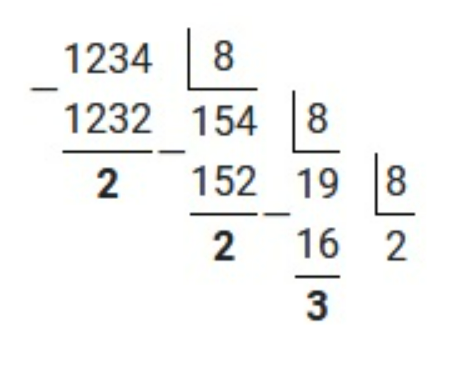
\includegraphics[width=0.4\textwidth]{decimal_to_octal.png}
\caption{Пример перевода десятичных чисел в восьмиричную систему счисления.}
\label{fig:example1}
\end{figure}

Второй алгоритм базируется на развернутой форме записи числа для позиционной системы счисления:
\label{Example:MathFont}
\begin{equation}\label{eq:1}
A_n = a_{n-1} * q^{n-1} + a_{n-2} * q^{n-2} + ... + a_0 * q^0\,;
\end{equation} 

где $A$ — число, $q$ — основание системы счисления, а $n$ — количество разрядов числа.

Зная, что 8 — основание системы счисления, выведем формулу перевода:
\label{Example:MathFont2}
\begin{equation}\label{eq:2}
A_8 = a_{n-1} * 8^{n-1} + a_{n-2} * 8^{n-2} + ... + a_0 * 8^0\,;
\end{equation}

\newpage
\begin{Example}\label{Example:MathFont3}
Перевод числа 7471 из восьмеричной системы в десятичную. 
\begin{equation*}\label{eq:3}
\begin{aligned}
7471_8= 7 * 8^3 + 4 * 8^2 + 7 * 8^1 + 1 * 8^0 = 7 * 512 + 4 * 64 + 7 * 8 + 1 * 1 = \\
3584 + 256 + 56 + 1 = 3897_{10}\,;
\end{aligned}
\end{equation*} 
\end{Example} 
\textbf{Ответ:} $7471_8 = 3897_{10}$ 

\vspace{1em}
Таким образом, \textbf{алгоритм перевода целого восьмеричного числа в десятичную систему счисления} состоит в том, чтобы число представить в виде суммы произведений степеней основания восьмеричной системы счисления на соответствующие цифры в разрядах восьмеричного числа.

\subsubsection{Новые алгоритмв перевода из одной позиционной системы в другую}
Новые алгоритмы перевода из десятичной системы счисления в восьмиричную и из восьмиричной системы счисления в десятичную были описаны в книгах <<Системы счисления и их применение>> ~\cite{CountSystems} и <<Занимательная компьютерная арифметика: Математика и искусство счета на компьютерах и без них>> ~\cite{ComputerArithm} профессора Гашкова С. Б.

Описанные в книгах методы представляют собой нестандартрные методы взаимного перевода десятичных и двоичных чисел, предложенные Соденом в 1953 году и Розье в 1962 году, и основанные на так называемой схеме Горнера. При этом в данных методах используются промежуточные переводы в восьмиричную систему счисления, что как раз отвечает поставленной перед нами задачей. Поэтмоу методами Содена и Розье можно осуществлять и только взаимный перевод десятичных и восьмеричных чисел. Ниже будут описаны алгоритмы взаимных переводов из восьмиричной системы в десятичную, и обратно.

\vspace{1em}
\textbf{Алгоритм перевода целых восьмеричных чисел в десятичную систему счисления.}

Для $n$-значного восьмиричного числа $u = (u_n...u_1)_8$ выполняются $(n - 1)$ шагов по переводу его в десятичную систему.

На $k$-м шаге выполняем над полученной на предыдущем шаге записью в десятичной арифметике действия:
\label{Example:MathFont4} 
\begin{equation*}\label{eq:4}
\begin{aligned}
\overline{u_n ... u_{n-k-1}} - 2 * \overline{u_n ... u_{n-k}} = \overline{v_{n+1} ... v_{n-k-1}}
\end{aligned}
\end{equation*} 

и получаем запись $\overline{v_{n+1} ... v_{n-k-1}.u_{n-k-2} ... u_1}$. При этом старшие разряды могут оказаться нулевыми и в реальных вычислениях участвовать не будут. Десятичную запись числа u получаем на $(n - 1)$-м шаге.

\begin{Example}\label{Example:MathFont5}
Перевод числа 3747 из восьмеричной системы в десятичную. 

$$
\begin{array}{r}
-
\begin{array}{r}
3.747\\
6\quad\quad\\
\end{array} \\
\hline
-
\begin{array}{r}
31.47\\
62\,\,\,\,\\
\end{array} \\
\hline
-
\begin{array}{r}
252.7\\
504\\
\end{array} \\
\hline
2023\,\,\,
\end{array}
$$
\end{Example} 
\textbf{Ответ:} $3747_8 = 2023_{10}$ 

В данном примере приведен процесс перевода четырехзначного восьмиричного числа в десятичную систему. Соответственно, перевод состоит из трех шагов.

На первом шаге необходимо из числа 3747, рассматривая его как десятичное, вычесть удвоенное произведение его первой цифры на 100 (на $10^{n-2}$).Отметим, что с целью экономии времени конечные нули можно не выписывать.

На втором шаге надо из полученной разности (также рассматривая ее как десятичную) вычесть удвоенное произведение двузначного числа, образованного первой и второй цифрами разности, на 10 (на $10^{n-3}$).

На третьем, в данном случае последнем, шаге вычитается удвоенное произведение трехзначного числа, образованного тремя первыми цифрами последней разности, на 1 (на $10^0$, или на $10^{n-4}$).

Полученное число и будет искомым десятичным.

Видно, что при переводе используются только умножение на два и вычитание. Именно по этой причине алгоритм получается значительно проще по числу операций, чем стандартный алгоритм с делением.

\vspace{1em}
\textbf{Алгоритм перевода целых десятичных чисел в восьмеричную систему счисления.}

Данный метод почти такой же, как описанный выше (только,
можно сказать, <<наоборот>>).

Для $n$-значного десятичного числа $u = (u_n...u_1)_{10}$ выполняются $(n - 1)$ шагов по переводу его в восьмеричную систему.

На $k$-м шаге над полученной на предыдущем шаге записью выполняем действия (умножение и сложение) в в восьмеричной арифметике:
\label{Example:MathFont6} 
\begin{equation*}\label{eq:5}
\begin{aligned}
\overline{u_n ... u_{n-k-1}} + 2 * \overline{u_n ... u_{n-k}} = \overline{v_{n+1} ... v_{n-k-1}}
\end{aligned}
\end{equation*} 

и получаем запись $\overline{v_{n+1} ... v_{n-k-1}.u_{n-k-2} ... u_1}$. При этом старшие $(n + 1)$-е разряды могут оказаться нулевыми и в реальных вычислениях участвовать не будут. Восьмиричную запись числа u получаем на $(n - 1)$-м шаге.

\begin{Example}\label{Example:MathFont7}
Перевод числа 2023 из десятичной системы в восьмеричную. 

$$
\begin{array}{r}
+
\begin{array}{r}
2.023\\
4\quad\quad\\
\end{array} \\
\hline
+
\begin{array}{r}
24.23\\
50\,\,\,\,\\
\end{array} \\
\hline
+
\begin{array}{r}
312.3\\
624\\
\end{array} \\
\hline
3747\,\,\,
\end{array}
$$
\end{Example} 
\textbf{Ответ:} $2023_{10} = 3747_8$ 

В данном случае разобран процесс перевода четырехзначного десятичного числа в восьмиричную систему, а сам перевод состоит из трех шагов. Основным нюансом данного алгоритма является проведение всех арифметических операций (умножение и сложение) в восьмиричной системе.

На первом шаге к числу 2023 прибавляется удвоенное произведение его первой цифры на 100 (на $10^{n-2}$). С целью экономии времени конечные нули могут быть опущены (не выписаны).

На втором шаге надо к полученной записи прибавляется удвоенное произведение двузначного числа, образованного первой и второй цифрами полученной на предыдущем шаге записи, на 10 (на $10^{n-3}$).

На третьем, в данном случае последнем, шаге складываются полученное на предыдущем шаге число и удвоенное произведение трехзначного числа, образованного тремя первыми цифрами последней полученной записи, на 1 (на $10^0$, или на $10^{n-4}$).

Итоговое число является искомым восьмиричным.

Отметим, что при переводе используются только умножение на два и сложение. Из-за отсутсвия операции деления данный алгоритм также получается проще по числу операций, чем стандартный алгоритм перевода десятичных чисел в восьмиричную систему счисления.

\subsubsection{Обоснвоание новых методов перевода десятичных и восьмеричных чисел}

Как было обозначено ранее, методы Содена и Розье были основаны на так называемой схеме Горнера. Опишем как данный алгоритм устроен и связан с методами перевода восьмиричных и десятичных чисел, на примерах обоснуем справедливость данных методов. 

Схема Горнера (или правило Горнера, метод Горнера, метод Руффини-Горнера) — это алгоритм вычисления значения многочлена, записанного в виде суммы мономов (одночленов), при заданном значении переменной. Также данный алгоритм применяется для вычисления частного и остатка от деления многочлена $p(x)$ на $x - a$.

Итак, пусть дан произвольный многочлен
в восьмеричной арифметике:
\label{Example:MathFont8} 
\begin{equation*}\label{eq:8}
\begin{aligned}
p(x) = u_n * x^n + ... + u_1 * x + u_0.
\end{aligned}
\end{equation*}

Деление этого многочлена на $x - a$ — это представление его в виде 
\label{Example:MathFont9} 
\begin{equation*}\label{eq:9}
\begin{aligned}
p(x) = (x - a) * h(x) + r,\,\,\,\qquad
h(x) = v_{n-1} * x^{n-1} + ... + v_1 * x + v_0.
\end{aligned}
\end{equation*}

Можно непосредственно проверить, что коэффициенты частного $h(x)$ можно найти по формулам 
\label{Example:MathFont10} 
\begin{equation*}\label{eq:10}
\begin{aligned}
v_{n-1} = u_n, v_{n-2} = u_{n-1} + a * v_{n-1}, ..., v_0 = u_1 + a* v_1, 
\end{aligned}
\end{equation*}
а остаток $r$ можно вычислить по формулам
\label{Example:MathFont11} 
\begin{equation*}\label{eq:11}
\begin{aligned}
r = u_0 + a*v_0 = u_0 + a*(u_1 + a*v_1) = u_0 + a*(u_1 + a*(u_2 + a*v_2)) = ... \\
= u_0 + a*(u_1+a*(...(u_{n-1}+a*u_n)...) = u_n*a^n+...+u_1*a+u_0 = p(a).
\end{aligned}
\end{equation*}
Описанный выше метод вычисления и называется схемой Горнера.

Теперь по порядку опишем взаимосвязь рассмотренных алгоритмов перевода Содена и Розье со схемой Горнера. 

Напомним, что в алгоритме перевода целых восьмеричных чисел в десятичную систему счисления, предложенном Соденом, на каждом шаге полученное число рассматривается как десятичное. Тогда, воспользуясь схемой Горнера, представим число 3747 из примера \ref{Example:MathFont5} следующим образом:
\label{Example:MathFont12} 
\begin{equation*}\label{eq:12}
\begin{aligned}
3747_{10} = 3 * 10^3 + 7 * 10^2 + 4 * 10 + 7 = ((3 * 10 + 7)*10 + 4) * 10 + 7. 
\end{aligned}
\end{equation*}

Вспомним, что по стандартному алгоритму восьмиричное число переводится в десятичное в помощью развернутой формы записи числа, а именно:
\label{Example:MathFont13} 
\begin{equation}\label{eq:13}
\begin{aligned}
3747_8 = 3 * 8^3 + 7 * 8^2 + 4 * 8 + 7. 
\end{aligned}
\end{equation}
А теперь, воспользовавшись схемой Горнера и тем фактом, что $8=10-2$ перепишем (\ref{eq:13}):

\label{Example:MathFont14} 
\begin{equation*}\label{eq:14}
\begin{aligned}
3747_8 = 3 * (10-2)^3 + 7 * (10-2)^2 + 4 * (10-2) + 7 = \\
= ((3 * (10-2) + 7)*(10-2) + 4) * (10-2) + 7. 
\end{aligned}
\end{equation*}
Видно, откуда в алгоритм Содена появилось вычитание удвоенного числа. Если рассматривать каждую скобку по отдельности, то можно проследить каждый шаг алгоритма, описанного ранее. Например, первая скобка $(3 * (10-2) + 7)$ соответствует первому шагу алгоритма, когда из числа 3747 вычитается шестерка, т.е. удвоенная первая цифра 3. Действительно, $(3 * (10-2) + 7) = 3*10 - 6 + 7 = 31$.
В результате первого шага получаем число 31, которое является двузначным числом из той самой разности, полученной после первого шага алгоритма Содена, и которое на втором шаге будет удвоенно и вычтено из полученной разности.

Аналогично рассматривается оставшаяся запись из уравнения (3). В итоге, действительно, получаем верное десятичное число: 
\label{Example:MathFont15} 
\begin{equation*}\label{eq:15}
\begin{aligned}
3747_8 = ((3 * (10-2) + 7)*(10-2) + 4) * (10-2) + 7 = \\
= 3 * 8^3 + 7 * 8^2 + 4 * 8 + 7 = 1536 + 448 + 32 + 7 = 2023_{10}. 
\end{aligned}
\end{equation*}

Наконец перейдем к алгоритму Розье. Так же воспользуемся схемой Горнера и представим число 2023 из примера \ref{Example:MathFont7} следующим образом:
\label{Example:MathFont16} 
\begin{equation*}\label{eq:16}
\begin{aligned}
2023_{10} = 2 * 10^3 + 0 * 10^2 + 2 * 10 + 2 = ((2 * 10 + 0)*10 + 2) * 10 + 3. 
\end{aligned}
\end{equation*}
Теперь представляем 10 в виде суммы 8 и 2:

\label{Example:MathFont17} 
\begin{equation*}\label{eq:17}
\begin{aligned}
2023_{10} = ((2 * (8+2) + 0)*(8+2) + 2) * (8+2) + 3. 
\end{aligned}
\end{equation*}
Стало видно откуда появилось сложение удвоенного числа в алгоритме Розье. 

Напомним, что в новом алгоритме перевода десятичного числа в восьмиричную систему арифметика выполняется в восьмиричной системе. С учетом этого нюанса рассмотриваем каждую скобку полученного уравнения по отдельности:
\begin{enumerate}
    \item $(2 * (8+2) + 0) = 2 * 8 + 2 * 2 + 0 = 20 + 4 + 0 = 24$
    \item $((2 * (8+2) + 0)*(8+2) + 2) = 24 *(8+2) + 2 = 240 + 50 + 2 = 312$
    \item $((2 * (8+2) + 0)*(8+2) + 2) * (8+2) + 3 = 312 * (8 + 2) + 3 = 3120 + 629 + 3 = 3747$
\end{enumerate}
Наглядно видно, что в результате первого шага получаем число 24, которое является двузначным числом из той суммы, полученной после первого шага алгоритма Розье, и которое на втором шаге будет удвоенно и прибавлено к полученной сумме. Результатом второго шага является число 312, а в результате третьего, последнего, шага получено число 3747, являющееся восьмиричной записью десятичного числа 2023.

\subsection{Разработка и реализация}
Для достижения поставленных задач был реализован программный продукт на языке С. В результате была создана программа, которая генерирует числовые примеры заданной длины и запускает алгоритмы перевода в системы счисления.
\begin{listing}
\caption{Структуры, близкие структурам Рефала}
\label{lst:refal}
\begin{minted}[frame=single,fontsize = \footnotesize, linenos, breaklines = True, xleftmargin = 1.5em,breaksymbol = ""]{c}
/*** Refal structures. ***/
typedef struct link {
    char ptype; /* type of the link */  
    union {
        struct link *b; /* bracket: ptr to the pair */
    char *f; /* function or compound symbol: ptr to label. */
    char c; /* symbol: actual value. */
    /* unsigned long u; /+* unicode symbol */
    unsigned int u;  /* unicode symbol */
    unsigned long n; /*  macro-digit   */
    unsigned short us_1, us_2;
    } pair;
    struct link *prec; /* ptr to preceding link */
    struct link *foll; /* ptr to following link */
} LINK;
\end{minted}
\end{listing}

\subsubsection{Особенности программы}
Одной из особенностей программной реализации является проблема переполнения памяти в случае с большими числами, поскольку числа в системе $2^{64}$ необходимо хранить в структурах, близких структурам Рефала (см. Листинг 1), где макро-цифра имеет тип данных unsigned long. К сожалению число $2^{64}$ на ного больше максимально возможного числа типа unsigned long. Для решения проблемы было решено воспользоваться равенством $2^{64} = (2^{32})^2$. 

Данное равенство говорит о том, что цифры числа N в системе счисления по основанию $2^{64}$ строятся следующим образом: начиная с младших разрядов, макро-цифра числа N по основанию $2^{64}$ есть последовательность двух макро-цифр этого же числа по основанию $2^{32}$. В таком случае, нечетные макроцифры по основанию $2^{32}$ укладываются в младшую половину макро-цифры по основанию $2^{64}$, а четные -- в старшую половину.

При использовании такой техники было необходимо реализовать взаимный перевод восьмиричных и двоичных чисел, двоичных чисел и чисел по основанию $2^{32}$, а также заполнение структур, близких структурам Рефала в соответствии описанным выше методом.

Другой важной особенностью программы являеся модификация нового алгоритма перевода из десятичной системы счисления в восьмиричную. Вопрос о модификации алгоритма был рассмотрен в процессе тестирования первой версии программы. Было замечено, что в новом алгоритме в книгах \cite{CountSystems} и \cite{ComputerArithm}, которые были использованы в качестве источника, представлены примеры только для тех чисел, у которых в старшем разряде стоит цифра от 1 до 4. Таким образом, на первом шаге алгоритма при умножении на два в результате не получается двузначное число, и ,соответственно, на каждом шаге алгоритма не возникает ситуации, при которой число-результат увеличивалось бы в длине. Однако с числами, начиньающимися на цифру от 5 до 9 описанный в книгах алгоритм давал сбой.

Решение проблемы было выявлено в процессе экспериментов с различными входными данными. При этом стабильно прослеживалось то, что на каждом шаге результат умножения на 2 необходимо записывать для последующего сложения так, что его последняя цифра стоит сразу за точкой, отделяющей число, которое мы умножали. То есть удвоенное число сдвигается относительно цифр исходного числа, на которое мы умножали, вправо ровно на одну цифру.

В итоге, алгоритм был модифицирован следующим образом: 

На $k$-м шаге над полученной на предыдущем шаге записью выполняем действия (умножение и сложение) в в восьмеричной арифметике и при этом следим за результатом умножения на два:
\begin{enumerate}
    \item если получается число, длина которого не изменилась (например, у $2$ длина единица, и $2*2 =4_8$ также имеет длину 1), тогда результат умножения записывается в столбик под исходное число, начиная со второго после старшего разряда исходного.
    \item если получается число, длина которого больше, изначального (например, у $6$ длина единица, и $6*2 =14_8$ имеет длину 2), тогда результат умножения записывается в столбик под исходное число, начиная со старшего разряда исходного.
\end{enumerate}

Более того, на каждом шаге необходимо следить за значением суммы исходного числа с удвоенным:
\begin{enumerate}
    \item если после сложения получается число, длина которого не изменилась (например, после первого шага для числа $6297$, получаем $7697$ - длина 4, так же как и у $6297$), тогда результат сложения записывается записывается в столбик под исходное число, как обычно.
    \item если после сложения получается число, длина которого больше, чем длина изначального (например, после второго шага для числа $6297$ получаем $11657$ - длина 5), то происходит сдвиг самого числа-результата влево, тогда точка <<как бы>> передвигается не на одну позицию вправо, а на две позиции.
\end{enumerate}

Данные рассуждения проиллюстрированы на примере ниже:


\begin{Example}\label{Example:MathFont18}
Перевод числа 6297 из десятичной системы в восьмеричную. 

$$
\begin{array}{r}
+
\begin{array}{r}
6.297\\
14\,\,\,\,\,\,\,\,\\
\end{array} \\
\hline
+
\begin{array}{r}
76.97\\
174\,\,\,\,\,\,\\
\end{array} \\
\hline
+
\begin{array}{r}
1165.7\\
2353\\
\end{array} \\
\hline
14231\,\,\,
\end{array}
$$
\end{Example} 
\textbf{Ответ:} $6297_{10} = 14231_8$ 

Посняим данный пример, используя схему Горнера.
\label{Example:MathFont19} 
\begin{equation*}\label{eq:19}
\begin{aligned}
6297_{10} = ((6*10 + 2)*10 +9)*10 + 7 = \\
= ((6*(8+2) + 2)*(8+2) +9)*(8+2) + 7.
\end{aligned}
\end{equation*}

Как и в предыдущих примерах, рассмотрим каждую скобку отдельно:
\begin{enumerate}
    \item $(6*(8+2) + 2) = 6 * 8 + 6 * 2 + 2 = 60 + 14 + 2 = 62 + 14 = 76_8$
    
    Видим, что результат умножения $6$ на $2$ является двузначным, поскольку мы работаем в восьмиричной системе и $6 * 2 = 14_8$, соответственно возникает перенос единицы в старший разряд.
    \item $((6*(8+2) + 2)*(8+2) +9) = 76 *(8+2) + 9 = 76 * 8 + 76 * 2 + 9 = 760 + 174 + 9 =  769 + 174 = 1165_8$
    
    На втором шаге также результат умножения $76$ на $2$ имеет большую длину, является трехзначным, поскольку мы в восьмиричной системе и $76 * 2 = 174_8$, соответственно возникает перенос единицы в старший, третий, разряд.
    \item $((6*(8+2) + 2)*(8+2) +9)*(8+2) + 7 = 1165 * (8 + 2) + 7 = 1165 * 8 + 1165 * 2 + 7 = 11650 + 2352 + 7 =  11657 + 2352 = 14231_8$
    
    Мы видим, что $11657$, полученное после второго шага алгоритма, отличается по длине от результата $7697$, поулченного на первом шаге. Именно в таком случае и происходит так называемый сдвиг влево, он обоснован простым переносом в старший разряд, который возникает в связи с использованием восьмиричной арифметики.
\end{enumerate}
\vspace{0.2em}
В конечном итоге, получен верный результат $14231_8$.

С учетом всех описанных выше особенностей программа была скорректирована. Основные функции проекта, необходимые для перевода чисел в различные системы счисления, приведены в листингах 2-8 в приложении А.


\subsubsection{Тестирование}
Целью тестирования являлось желание получить подтверждение или опровержение гипотезы о том, что новые алгоритмы взаимного перевода из систем счисления имеют меньшее время выполнения, по сравнению со стандартными алгоритмами.

Реализованная программа была протестирована на входных десятичных числах разной длины. Результаты были систематизированы в сравнительные таблицы ~\ref{table:table11} и ~\ref{table:table22}.

\begin{table}[!htb]
\caption{\centering Время работы стандартного и нового алгоритмов перевода из 10-й системы в систему счисления по основанию $2^{64}$.}
\small
\centering\begin{tabular}{|c|c|c|}
\hline
\multirow{ 2}{*}{Входное десятичное \vspace{2em}} & \multirow{ 2}{*}{Время выполнения стандартного \vspace{2em}} & \multirow{ 2}{*}{Время выполнения \vspace{2em}} \\
число & алгоритма, с. & нового алгоритма, с.\\
\hline
123 & 0.012 & 0.001 \\
\hline
\end{tabular}
\label{table:table11}
\end{table}

\begin{table}[!htb]
\caption{\centering Время работы стандартного и нового алгоритмов перевода из системы по основанию $2^{64}$ в 10-ю систему счисления.}
\small
\centering\begin{tabular}{|c|c|c|c|}
\hline
\multirow{ 2}{*}{Входное десятичное \vspace{2em}} & \multirow{ 2}{*}{Время выполнения стандартного \vspace{2em}} & \multirow{ 2}{*}{Время выполнения \vspace{2em}} \\
число & алгоритма, с. & нового алгоритма, с.\\
\hline
123 & 0.012 & 0.001 \\
\hline
\end{tabular}
\label{table:table22}
\end{table}


\anonsection{ЗАКЛЮЧЕНИЕ} %Заключение
В результате практики поставленные задачи были успешно выполнены, и была создана программа, реализующая сравнение нового и стандартного алгоритма перевода натуральных чисел из десятичной системы счисления в систему счисления по основанию $2^{64}$. 

В процессе выполнения поставленной задачи были изучены и реализованы алгоритмы перевода из одной позиционной системы счисления в другую с использованием схемы Горнера. В ходе разработки был получен опыт работы с языком программирования Си. Результаты работы подтвердили поставленую гипотезу об оптимальности нового алгоритма без деления. 

В дальнейшем видится совершенствование проекта, его тестирование и внедрение описанных алгоритмов в Рефал-5 для оптиммальной работы с натуральными числами.

\newenvironment{code}{\captionsetup{type=listing}}{}

\newpage
\settocdepth{section}
\anonsection{ПРИЛОЖЕНИЕ А}
\vspace{-20pt}
\begin{code}
\caption{Новый алгоритм. Перевод десятичного числа в восьмиричную систему. Умножение на 2 в восьмиричной системе}
\vspace{10pt}
\label{lst:mul2octal}
\begin{minted}[frame=single,fontsize = \footnotesize, linenos, breaklines = True, xleftmargin = 1.5em,breaksymbol = "", escapeinside=``]{c}
char* mul_x_2_octal(char* code, long n) {
    char c;
    int i;
    char* code1;
    code1 = malloc(n + 1);
    long digit, dec, res;
    long carry = 0;
    code1[0] = '0';
    for (i = n - 1; i >= 0; i--) {
        c = code[i];
        char *pChar = &c;
        digit = (long)atoi(pChar); 
        digit = digit * 2;
        dec = digit / 8;
        res = digit%8 + carry;
        if (res > 9) {
            dec = res /8;
            code1[i + 1] = (res%10) + '0';
        } else {
            code1[i + 1] = res + '0';
        }
        if (dec > 0) {
            carry = dec;
        } else {
            carry = 0;
        }
    }
    if (i == -1 && carry > 0) {
        code1[0] = (long)(code1[0] - '0') + carry + '0';
    }
    code1[n+1] = '\0';
    return code1;
}
\end{minted}
\end{code}


\newpage
\begin{code}
\caption{Новый алгоритм. Перевод десятичного числа в восьмиричную систему. Сложение в восьмиричной системе}
\label{lst:octaladd}
\begin{minted}[frame=single,fontsize = \footnotesize, linenos, breaklines = True, xleftmargin = 1.5em,breaksymbol = "", escapeinside=``]{c}
char* my_octal_add(char* code1, char* code2, long n) {
    char *code;
    char c1, c2;
    int digit, digit1, digit2, sd, dec, res, carry = 0;
    code = malloc(n);
    unsigned long long i, len1 = strlen(code1), len2 = strlen(code2);
    c1 = code1[0];
    sd = c1-'0';
    code[0] = sd + '0';
    if (len1 == len2) {
        for (i = len1 - 1; i > 0; i--) {
            c1 = code1[i];
            c2 = code2[i];
            digit1 = c1-'0'; 
            digit2 = c2-'0'; 
            digit = digit1 + digit2;
            dec = digit / 8;
            res = digit%8 + carry;
            if (res > 7) {
                dec = res /8;
                code[i] = (res%8) + '0';
            } else {
                code[i] = res + '0';
            }
            if (dec > 0) {
                carry = dec;
            } else {
                carry = 0;
            }
            if (dec > 0 && i == 1) {
                code[0] = sd + carry + '0';
            }
        } 
        if (sd != 0) {
            code[0] = sd + (code2[0] - '0') + carry + '0';
        }
        code[n] = '\0';
        return code;
    }

    for (i = n - 1; i > len2; i--) {
        code[i] = code1[i];
    }
    for (i = len2; i > 0; i--) {
        c1 = code1[i];
        c2 = code2[i - 1];
        digit1 = c1-'0'; 
        digit2 = c2-'0'; 
        digit = digit1 + digit2;
        dec = digit / 8;
        res = digit%8 + carry;
        if (res > 7) {
            dec = res /8;
            code[i] = (res%8) + '0';
        } else {
            code[i] = res + '0';
        }
        if (dec > 0) {
            carry = dec;
        } else {
            carry = 0;
        }
        if (dec > 0 && i == 1) {
            code[0] = sd + carry + '0';
        }
    } 
    code[n] = '\0';
    return code;
}
\end{minted}
\end{code}

\newpage
\begin{code}
\caption{Новый алгоритм. Перевод восьмиричного числа в десятичную систему. Умножение на 2 в десятичной системе}
\label{lst:octaladd}
\begin{minted}[frame=single,fontsize = \footnotesize, linenos, breaklines = True, xleftmargin = 1.5em,breaksymbol = "", escapeinside=``]{c}
char* mul_x_2(char* code, long n) {
    char c;
    int i;
    char* code1;
    code1 = malloc(n + 1);
    long digit, dec, res;
    long carry = 0;
    code1[0] = '0';
    for (i = n - 1; i >= 0; i--) {
        c = code[i];
        char *pChar = &c;
        digit = (long)atoi(pChar); 
        digit = digit * 2;
        dec = digit / 10;
        res = digit%10 + carry;
        if (res > 9) {
            dec = res / 10;
            code1[i + 1] = (res%10) + '0';
        } else {
            code1[i + 1] = res + '0';
        }
        if (dec > 0) {
            carry = dec;
        } else {
            carry = 0;
        }
    }
    if (i == -1 && carry > 0) {
        code1[0] = (long)(code1[0] - '0') + carry + '0';
    }
    code1[n+1] = '\0';
    return code1;
}
\end{minted}
\end{code}

\newpage
\begin{code}
\caption{Новый алгоритм. Перевод восьмиричного числа в десятичную систему. Вычитание в десятичной системе}
\label{lst:octaladd}
\begin{minted}[frame=single,fontsize = \footnotesize, linenos, breaklines = True, xleftmargin = 1.5em,breaksymbol = "", escapeinside=``]{c}
char* my_decimal_sub(char* code1, char* code2, long n) {
    char *code;
    int digit, digit1, digit2, sd, dec, res, carry = 0;
    code = malloc(n + 1);
    sd = code1[0] - '0'; 
    code[0] = sd + '0';
    for (int i = n - 1; i > 0; i--) {
        digit1 = code1[i]-'0'; 
        digit2 = code2[i]-'0'; ;
        digit = digit1 - digit2 - carry;
        if (digit < 0) {
            carry = 1;
            code[i] = (digit + 10) + '0';
        } else {
            carry = 0;
            code[i] = digit + '0';
        }
        if (carry != 0 && i == 1) {
            code[0] = sd - carry + '0';
        }
    } 
    code[n] = '\0';
    return code;
}
\end{minted}
\end{code}

\newpage
\begin{code}
\caption{Стандартный алгоритм. Перевод из десятичной системы в восьмиричную систему.}
\label{lst:octaladd}
\begin{minted}[frame=single,fontsize = \footnotesize, linenos, breaklines = True, xleftmargin = 1.5em,breaksymbol = "", escapeinside=``]{c}
char* convert_from_decimal_to_octal(char* code, long n) {
    bool new_step = false;
    char* result;
    result = (char*)malloc((n + 2) * sizeof(char));
    int j = 0, d;
    char* code2;
    char* first_two_digits;
    first_two_digits = malloc(3);
    long digits, rem, quot, len = n;
    int first_digit = code[0] - '0', flag = 0;
    if (first_digit < 8) {
        slice(code, first_two_digits, 0, 2);
        first_two_digits[2] = '\0';
        digits = atol(first_two_digits);
        quot = digits / 8;
        rem = digits - quot * 8;
        flag = 1;
    } else {
        quot = first_digit / 8; 
        rem = first_digit - quot * 8; 
    }
    while( len != 1) {    
        if (new_step) {
            new_step = false;
            first_digit = code[0] - '0',
            flag = 0;
            if (first_digit < 8) {
                slice(code, first_two_digits, 0, 2);
                first_two_digits[2] = '\0';
                digits = atol(first_two_digits);
                quot = digits / 8;
                rem = digits - quot * 8;
                flag = 1;
                free(code2);
            } else {
                quot = first_digit / 8;
                rem = first_digit - quot * 8;
                flag = 0;
            }
        }
        int k = 0;
        code2 = malloc(len + 1);
        code2[k++] = (int)quot + '0';
        for (int i = 1; i < len; i++) {
            if (flag == 1) {
                i++;
                if (i == len) {
                    break;
                }
            } 
            d = code[i] - '0';
            flag = 0;
            if (rem != 0) {
                digits = rem * 10 + d;
                quot = digits / 8;
                rem = digits - quot * 8;
            } else {
                if (d < 8 && i != len - 1) {
                    code2[k++] = '0';
                    slice(code, first_two_digits, i, i + 2);
                    first_two_digits[2] = '\0';
                    digits = atol(first_two_digits);
                    quot = digits / 8;
                    rem = digits - quot * 8;
                    i++;
                } else {
                    quot = d / 8;
                    rem = d - quot * 8;
                }  
            }
            code2[k++] = (int)quot + '0';
        }
        result[j++] =  (int)rem + '0';
        new_step = true;
        code2[k] = '\0';
        memcpy(code, code2, k);
        len = k;
              
    }
    free(first_two_digits);
    if (len == 1) {
        d = code[0] - '0';
        while (d != 0) {
            if (d < 8) {
                result[j++] = d +'0';   
            } else {
                quot = d / 8;
                rem = d % 8;
                result[j++] = (int)rem + '0';
            }
            d = d/8;
        }
    }
    result[j++] =  '\0';
    free(code2);
    return result;
}
\end{minted}
\end{code}

\newpage
\begin{code}
\caption{Перевод из двоичной системы в систему по основанию $2^{32}$.}
\label{lst:octaladd}
\begin{minted}[frame=single,fontsize = \footnotesize, linenos, breaklines = True, xleftmargin = 1.5em,breaksymbol = "", escapeinside=``]{c}
unsigned long convert_to_2_in_32_system(char* code) {
    unsigned long res = 0;
    unsigned long cur;
    int deg = 0;
    int len = strlen(code);
    for (int i = len - 1; i >= 0; i--) {
        cur = code[i] - '0';
        res += cur * pow(2, deg);
        ++deg;
    }
    return res;
}
\end{minted}
\end{code}

\begin{code}
\caption{Заполнение структуры Рефала LINK.}
\label{lst:octaladd}
\begin{minted}[frame=single,fontsize = \footnotesize, linenos, breaklines = True, xleftmargin = 1.5em,breaksymbol = "", escapeinside=``]{c}
LINK* start_number = (LINK*)malloc(sizeof(LINK));
LINK* end_number;
LINK* prev_number;
prev_number = NULL;
bool flag_chetn = false;
unsigned long long old_len, len = strlen(binary);
while (len > 0) {
    LINK* number;
    number = (LINK*)malloc(sizeof(LINK));
    if (prev_number != NULL) {
        NEXT(prev_number) = number;
    }
    TYPE(number) = 'd';
    PREV(number) = prev_number;
    char* str = malloc(33 * sizeof(char));
    old_len = len;
    if (len >= 32) {
        slice(binary, str, len-32, len);
        len -= 32;
    } else {
        slice(binary, str, 0, len);
        len -= len;
    }
    
    PAIR(number).n = convert_to_2_in_32_system(str);
    if (old_len == strlen(binary)) {
        end_number = number;
    }
    free(str);
    prev_number = number; 
    flag_chetn = !flag_chetn;
}
    
if (len == 0) {
    if (flag_chetn) {
        LINK* number = (LINK*)malloc(sizeof(LINK));
        if (prev_number != NULL) {
            NEXT(prev_number) = number;
        }
        TYPE(number) = 'd';
        PREV(number) = prev_number;
        PAIR(number).n = 0;
        start_number = number;
    } else {
        start_number = prev_number;
    }
}
\end{minted}
\end{code}

\newpage
\begin{code}
\caption{Печать (в файл или стандартный поток вывода) чисел в системе счисления по основанию $2^{64}$.}
\label{lst:octaladd}
\begin{minted}[frame=single,fontsize = \footnotesize, linenos, breaklines = True, xleftmargin = 1.5em,breaksymbol = "", escapeinside=``]{c}
void print_Link_64(LINK* l, FILE* output) {
    if (output != NULL) {
        if (l != NULL && PREV(l) != NULL) {
            unsigned long senior = l->pair.n;
            unsigned long junior = l->prec->pair.n;
            char* macrodigit = malloc(40);
            char* jun = malloc(20);
            sprintf(macrodigit, "%ld", senior);
            sprintf(jun, "%ld", junior);
            strcat(macrodigit, jun);
            fputs(macrodigit, output);
            print_Link_64(l->prec->prec, output);
        }
    } else {
        if (l != NULL && PREV(l) != NULL) {
            unsigned long senior = l->pair.n;
            unsigned long junior = l->prec->pair.n;
            char* macrodigit = malloc(40);
            char* jun = malloc(20);
            sprintf(macrodigit, "%ld", senior);
            sprintf(jun, "%ld", junior);
            strcat(macrodigit, jun);
            printf("%s",macrodigit);
            print_Link_64(l->prec->prec, NULL);
        }
    }
}
\end{minted}
\end{code}

\renewcommand\refname{СПИСОК ИСПОЛЬЗОВАННЫХ ИСТОЧНИКОВ}
% Список литературы
\clearpage
%\bibliographystyle{ugost2008s}  %utf8gost71u.bst} %utf8gost705u} %gost2008s}
{\catcode`"\active\def"{\relax}
\addcontentsline{toc}{section}{\protect\numberline{}\refname}%
%\bibliography{biblio} %здесь ничего не меняем, кроме, возможно, имени bib-файла
\printbibliography
}
\newpage

\end{document}

